The intention of this report is to investigate preliminary data coming from the ITS and MFT in Run 3. The order of the discussion in this section will follow the order that we tackled things. This is done to show both the progression of our knowledge as well as to try to clarify some of the explanations in previous sections as the only way to truly understand some things is through example. 

\subsection{The Data}
The data analysed in this report was taken in October 2021, where protons were collided at a centre of mass energy of \SI{900}{\giga\electronvolt}. This is not an energy that we expect to use for physics research but it allows us to look at how the detectors are performing with more lightweight data, simply because there will be fewer particles created in the collisions and thus less data to work with. We are using runs 505548 and 505645. In this case, a run specifies a period of data taking for which all global settings remain the same. 



\subsection{Initial MFT Analysis}
In the AOD data model there is a table called \texttt{MFTTracks} which contains the tracks detected in the MFT. 

When we began this analysis, only two reconstruction passes had been run on the data and while the MFT was switched on for the runs, 

\begin{figure}[h]%
    \centering
    \begin{subfigure}[t]{.49\linewidth}
        \centering
        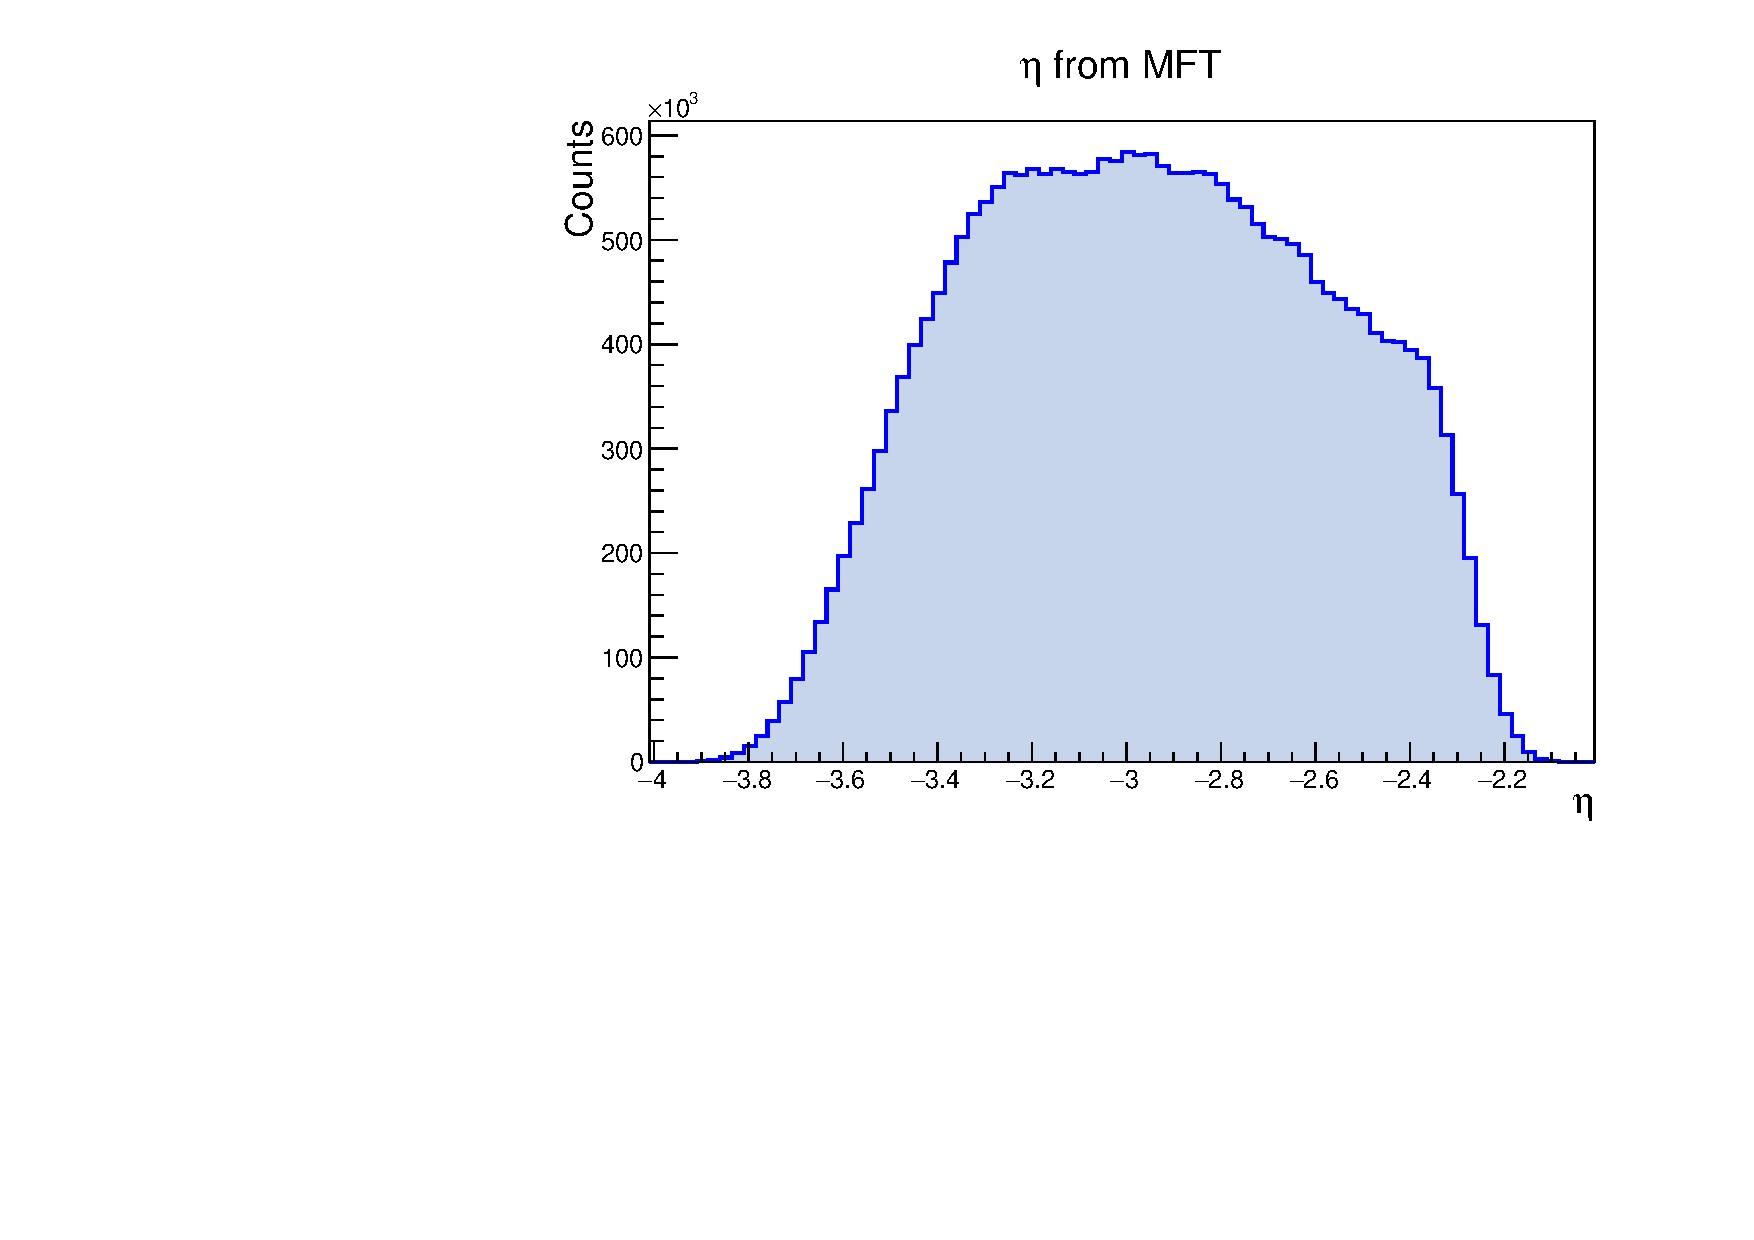
\includegraphics[width=\linewidth]{Plots/pass3_MFT/MFTeta_pass3.pdf}
        \caption{}
        \label{}
    \end{subfigure}
    \hfill
    \begin{subfigure}[t]{.49\linewidth}
        \centering
        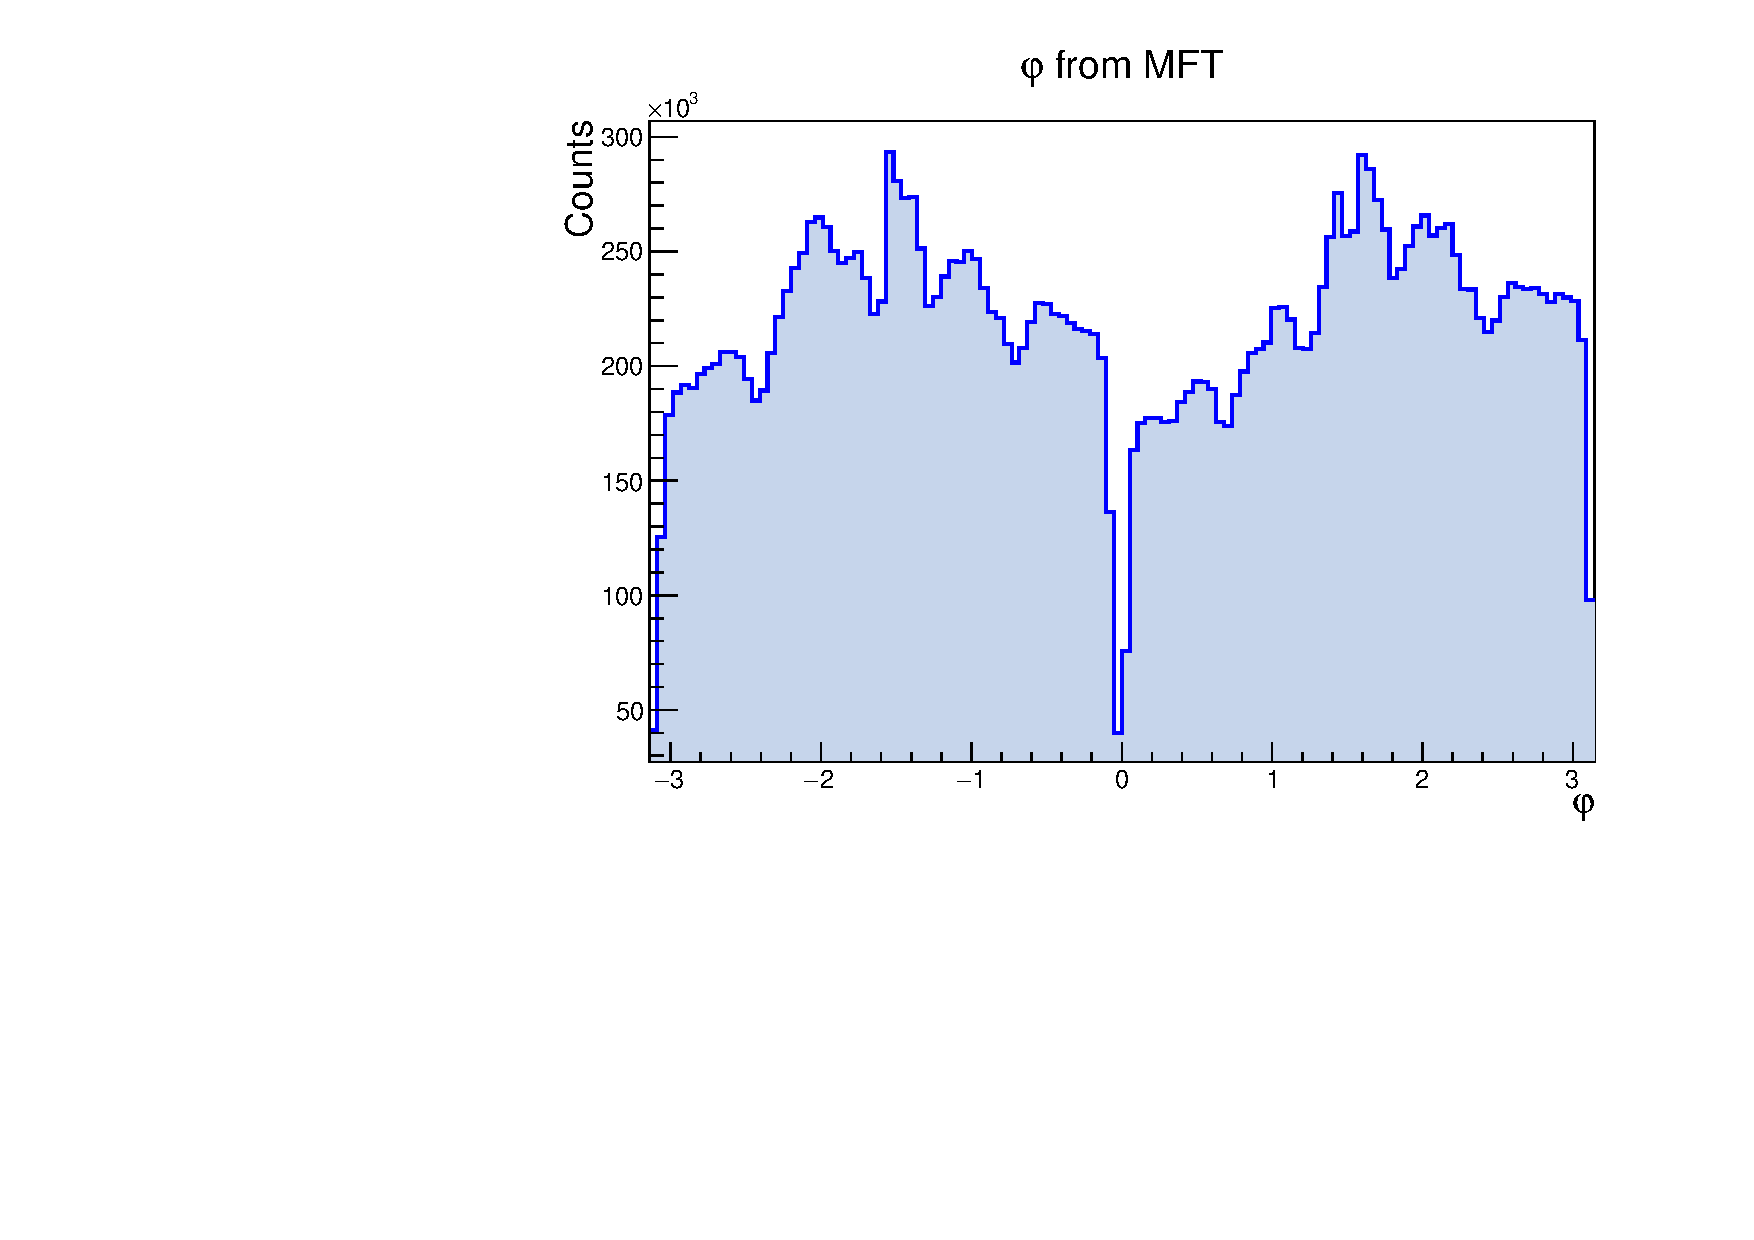
\includegraphics[width=\linewidth]{Plots/pass3_MFT/phi_pass3.pdf}
        \caption{}
        \label{}
    \end{subfigure}
    \begin{subfigure}[t]{.49\linewidth}
        \centering
        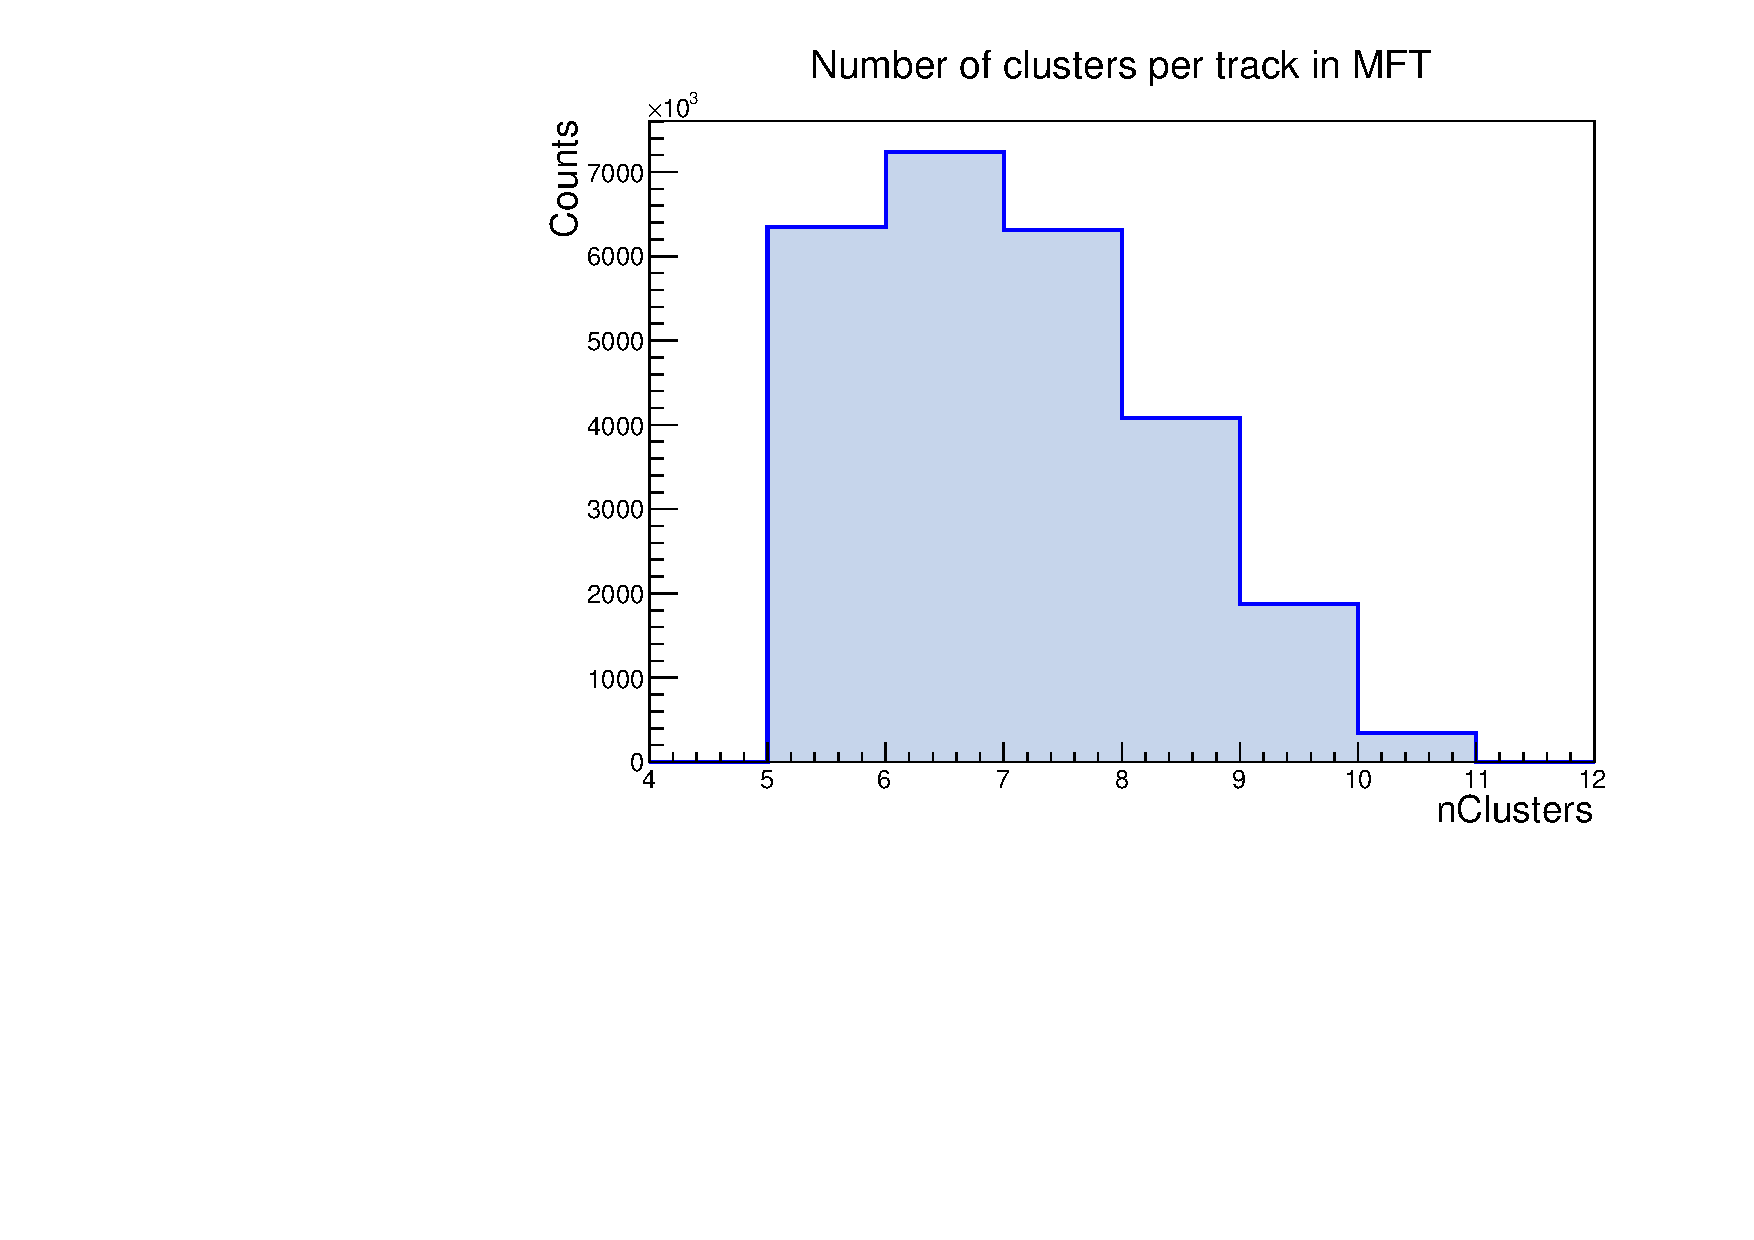
\includegraphics[width=\linewidth]{Plots/pass3_MFT/nClusters_pass3.pdf}
        \caption{}
        \label{}
    \end{subfigure}
    \hfill
    \begin{subfigure}[t]{.49\linewidth}
        \centering
        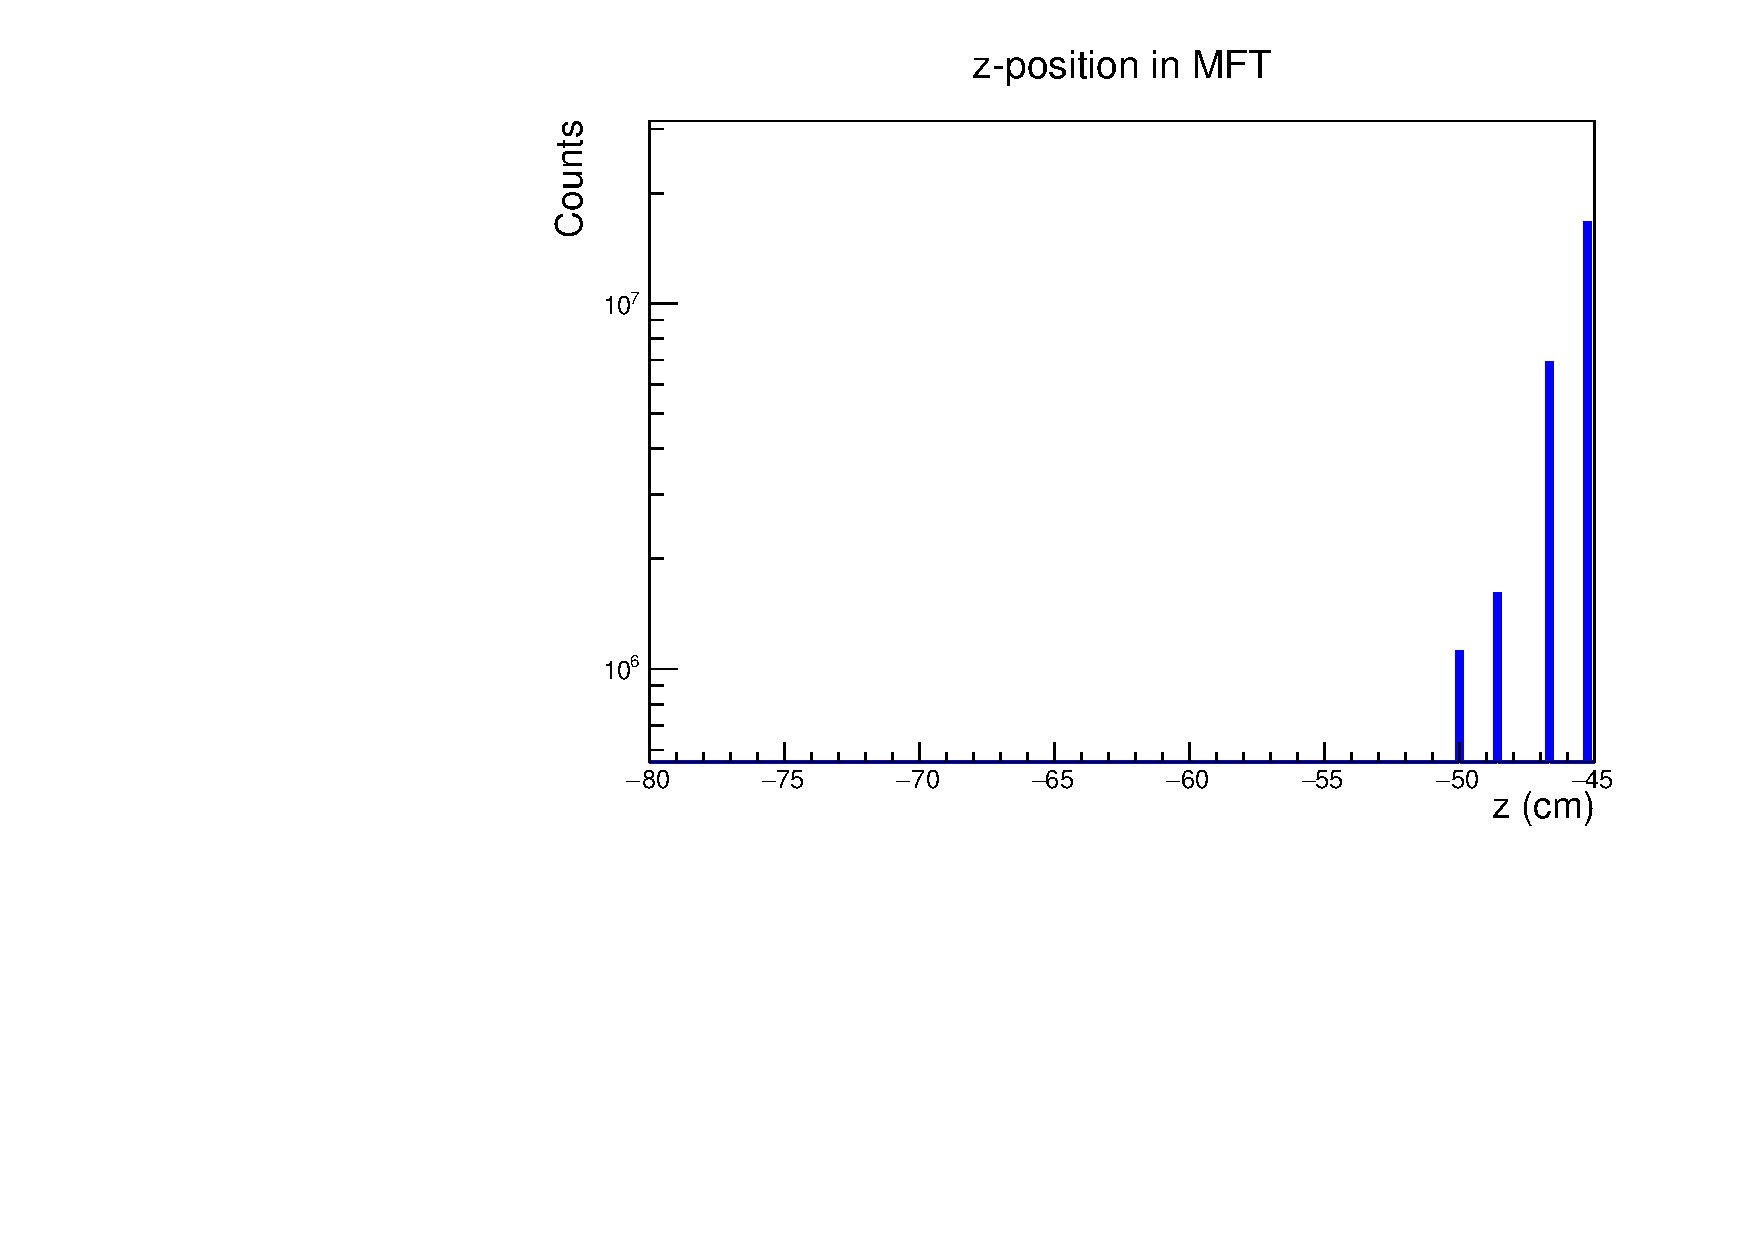
\includegraphics[width=\linewidth]{Plots/pass3_MFT/Z_MFT_pass3.pdf}
        \caption{}
        \label{}
    \end{subfigure}
\caption{}
\label{fig:MFT_1D_pass3}
\end{figure}

\begin{figure}[h]
    \begin{center}
        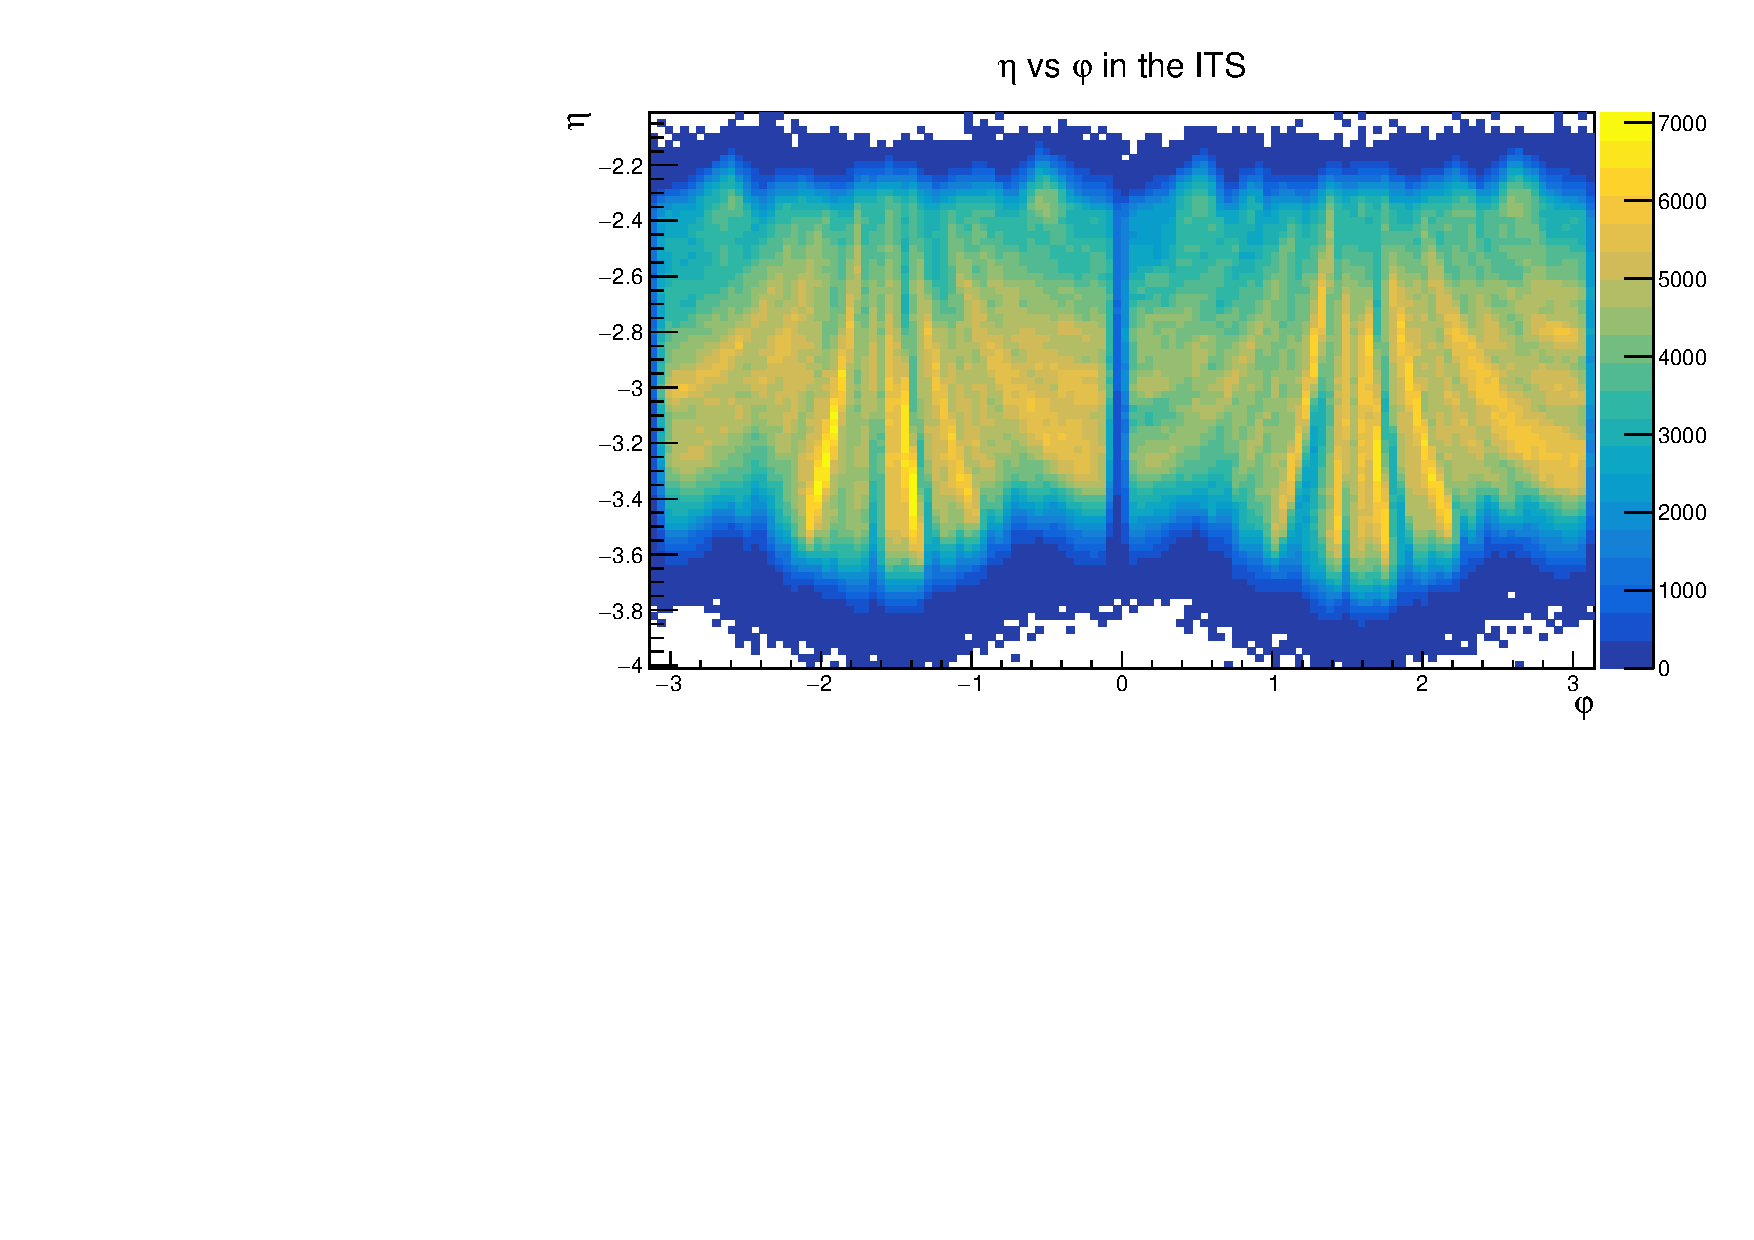
\includegraphics[width=.8\textwidth]{Plots/pass3_MFT/eta_phi_pass3.pdf}
        \caption{caption}
        \label{fig:eta_phi_pass3}
    \end{center}
\end{figure}


\begin{figure}[h]%
    \centering
    \begin{subfigure}[t]{.45\linewidth}
        \centering
        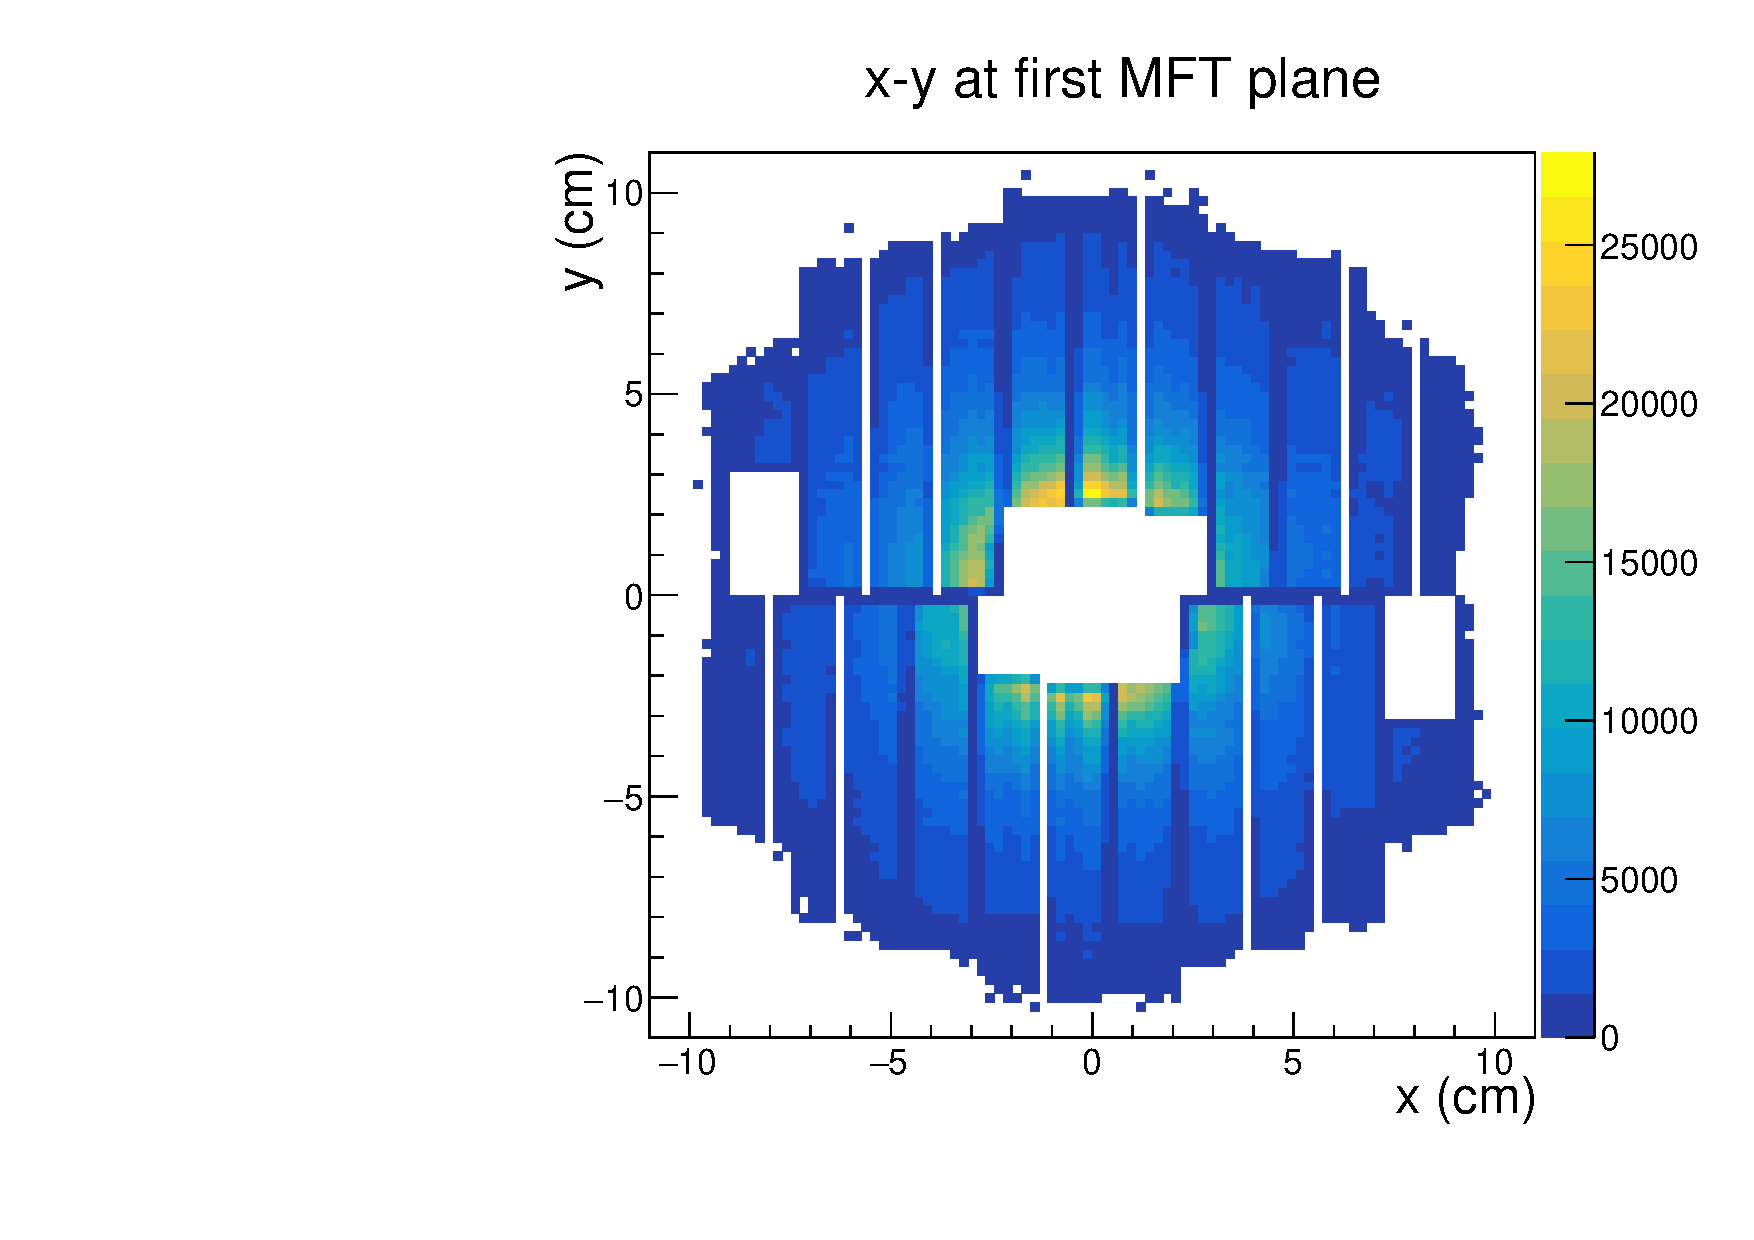
\includegraphics[width=\linewidth]{Plots/pass3_MFT/x_y_1_pass3.pdf}
        \caption{}
        \label{}
    \end{subfigure}
    \hfill
    \begin{subfigure}[t]{.45\linewidth}
        \centering
        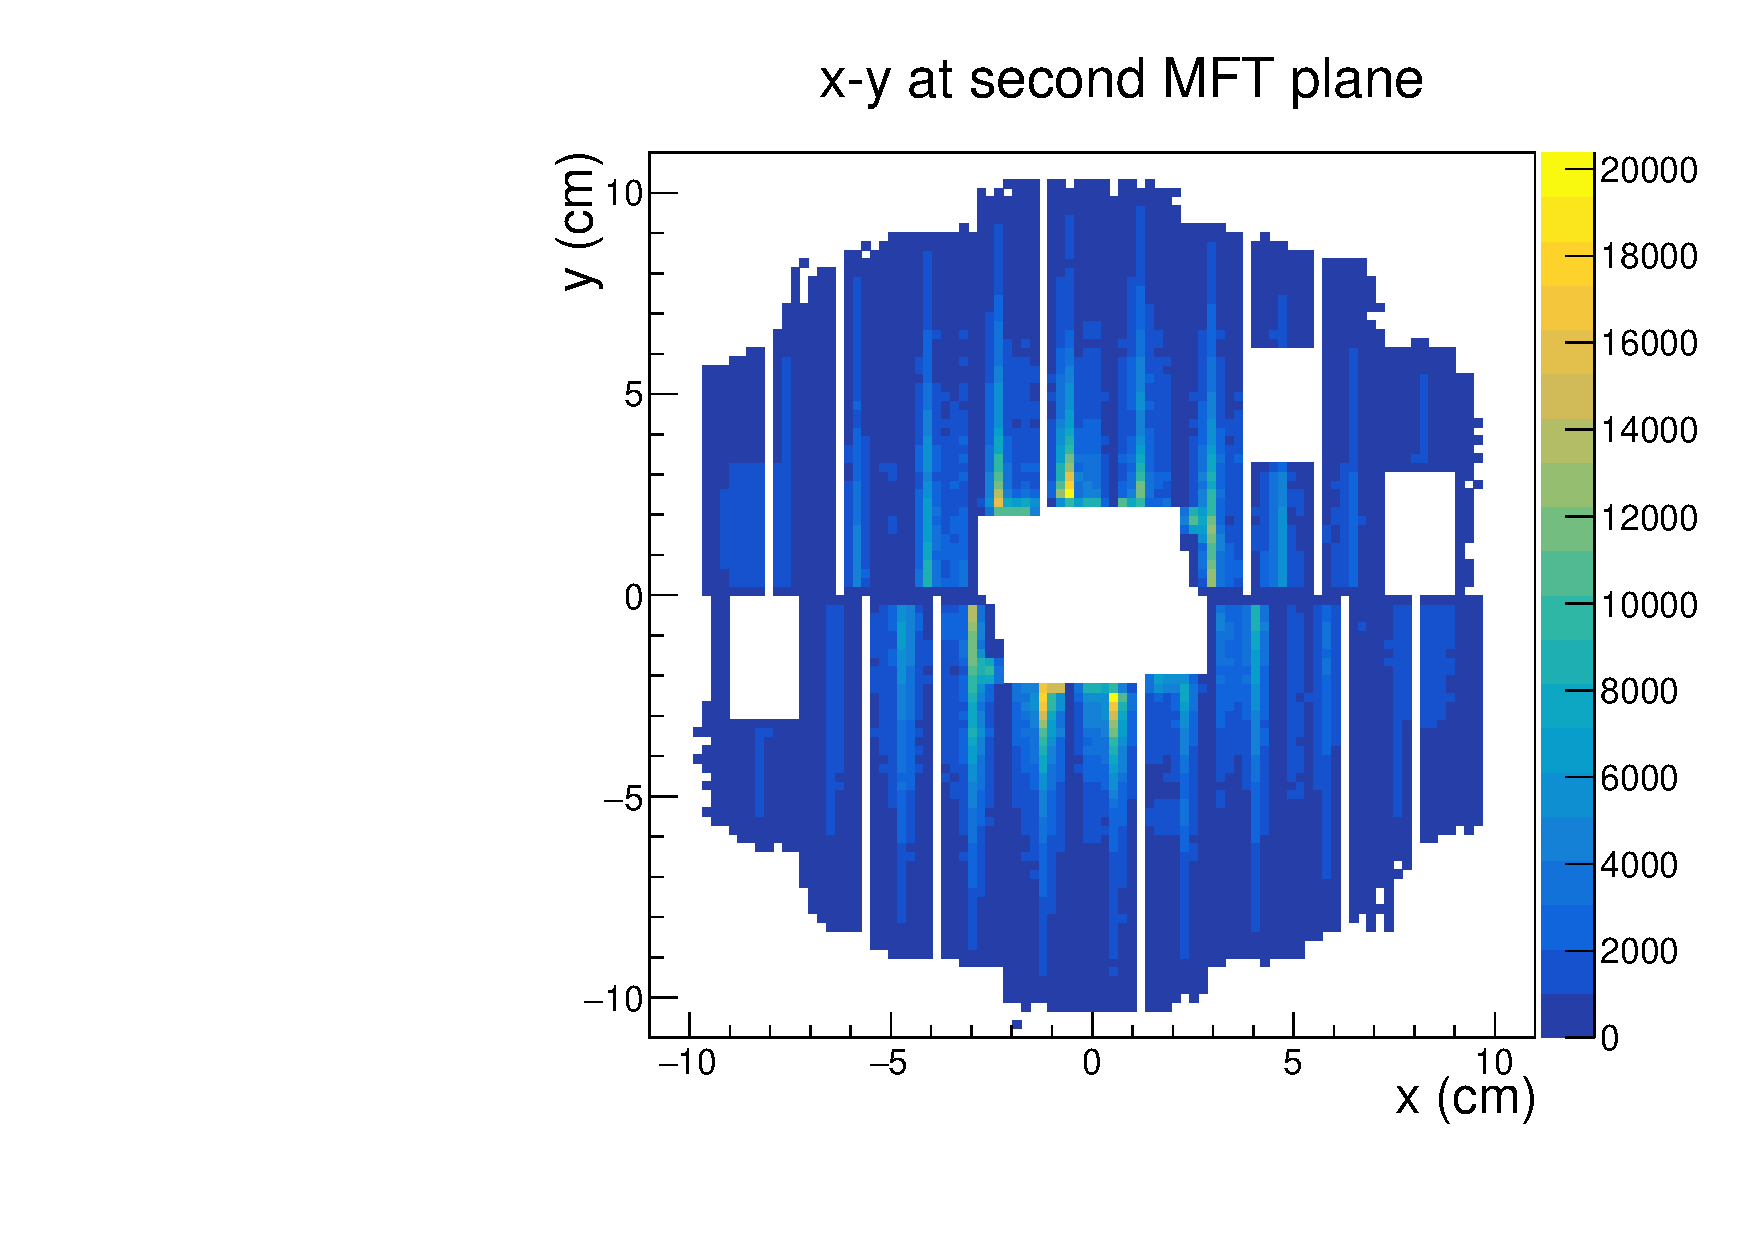
\includegraphics[width=\linewidth]{Plots/pass3_MFT/x_y_2_pass3.pdf}
        \caption{}
        \label{}
    \end{subfigure}
    \begin{subfigure}[t]{.45\linewidth}
        \centering
        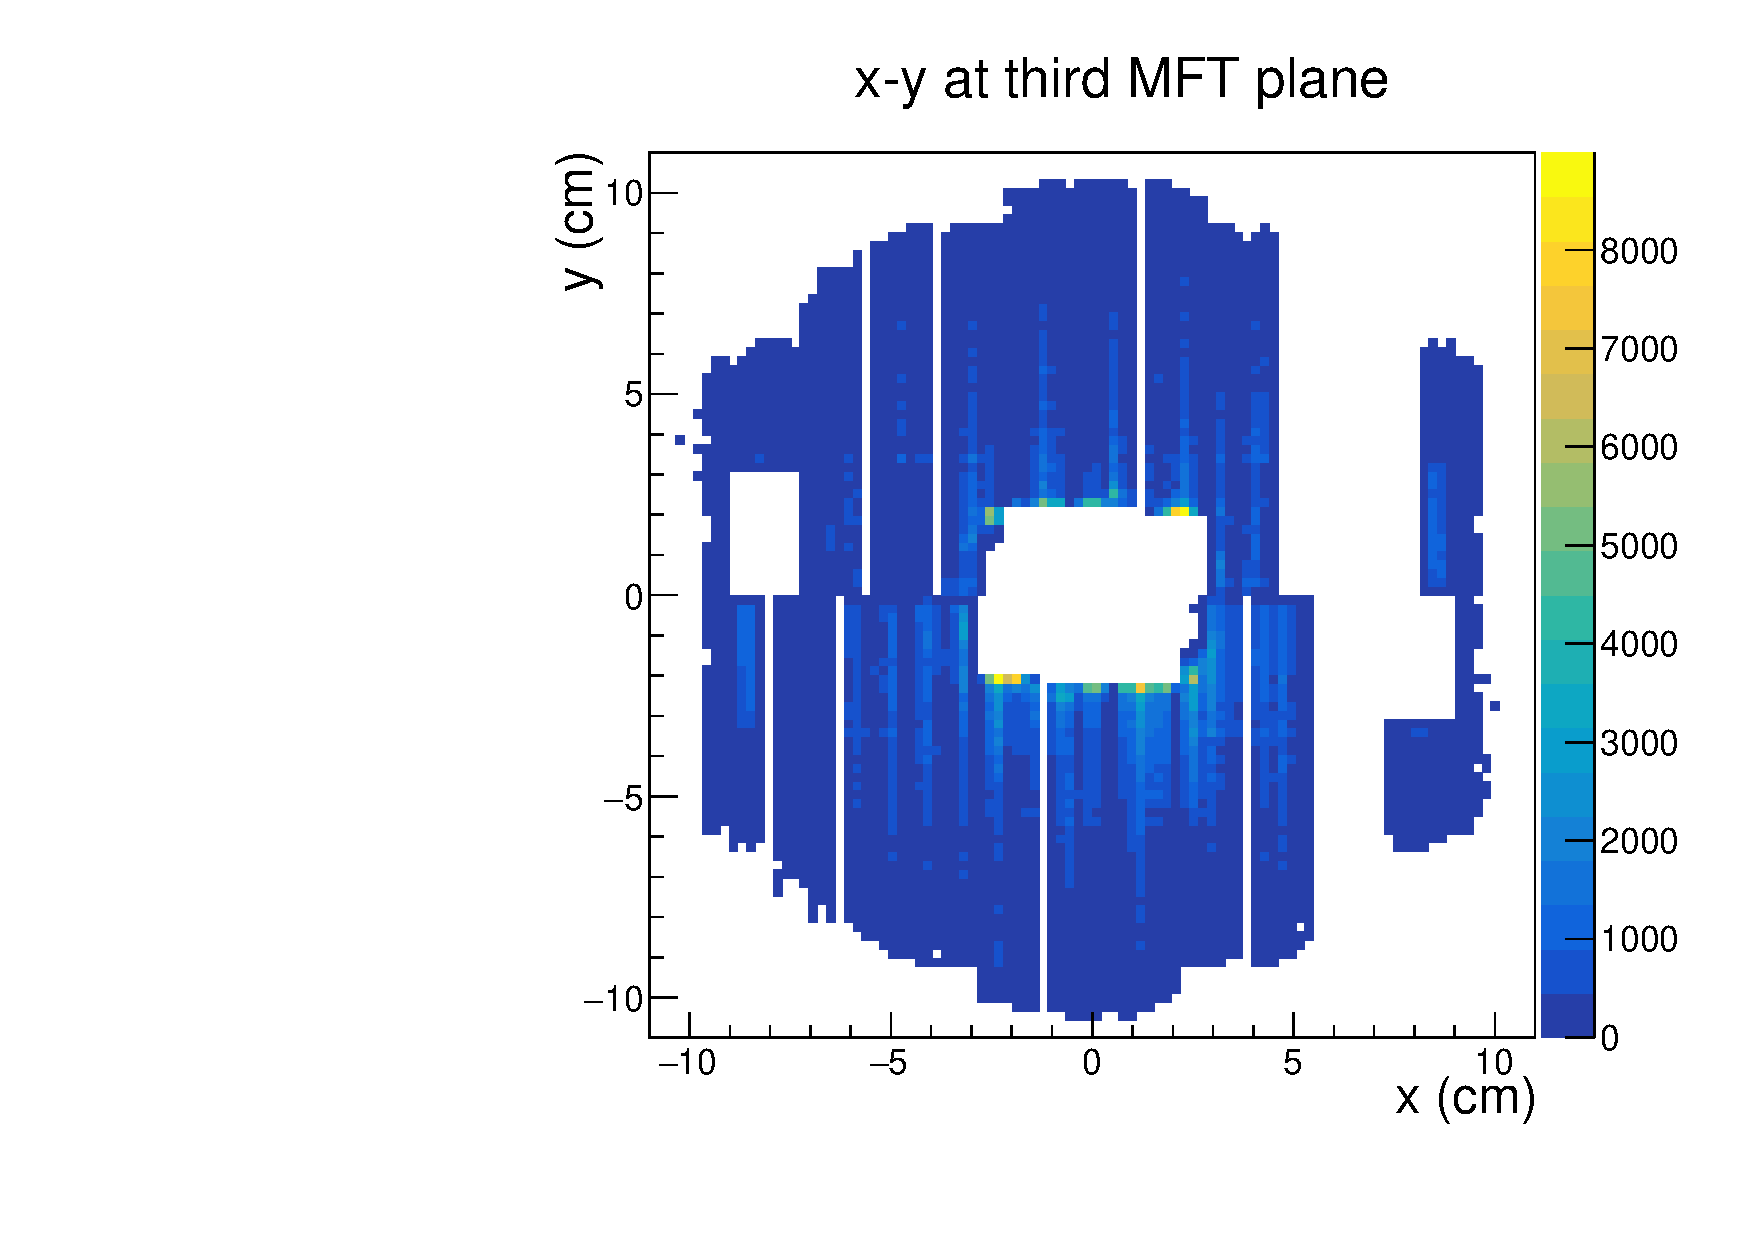
\includegraphics[width=\linewidth]{Plots/pass3_MFT/x_y_3_pass3.pdf}
        \caption{}
        \label{}
    \end{subfigure}
    \hfill
    \begin{subfigure}[t]{.45\linewidth}
        \centering
        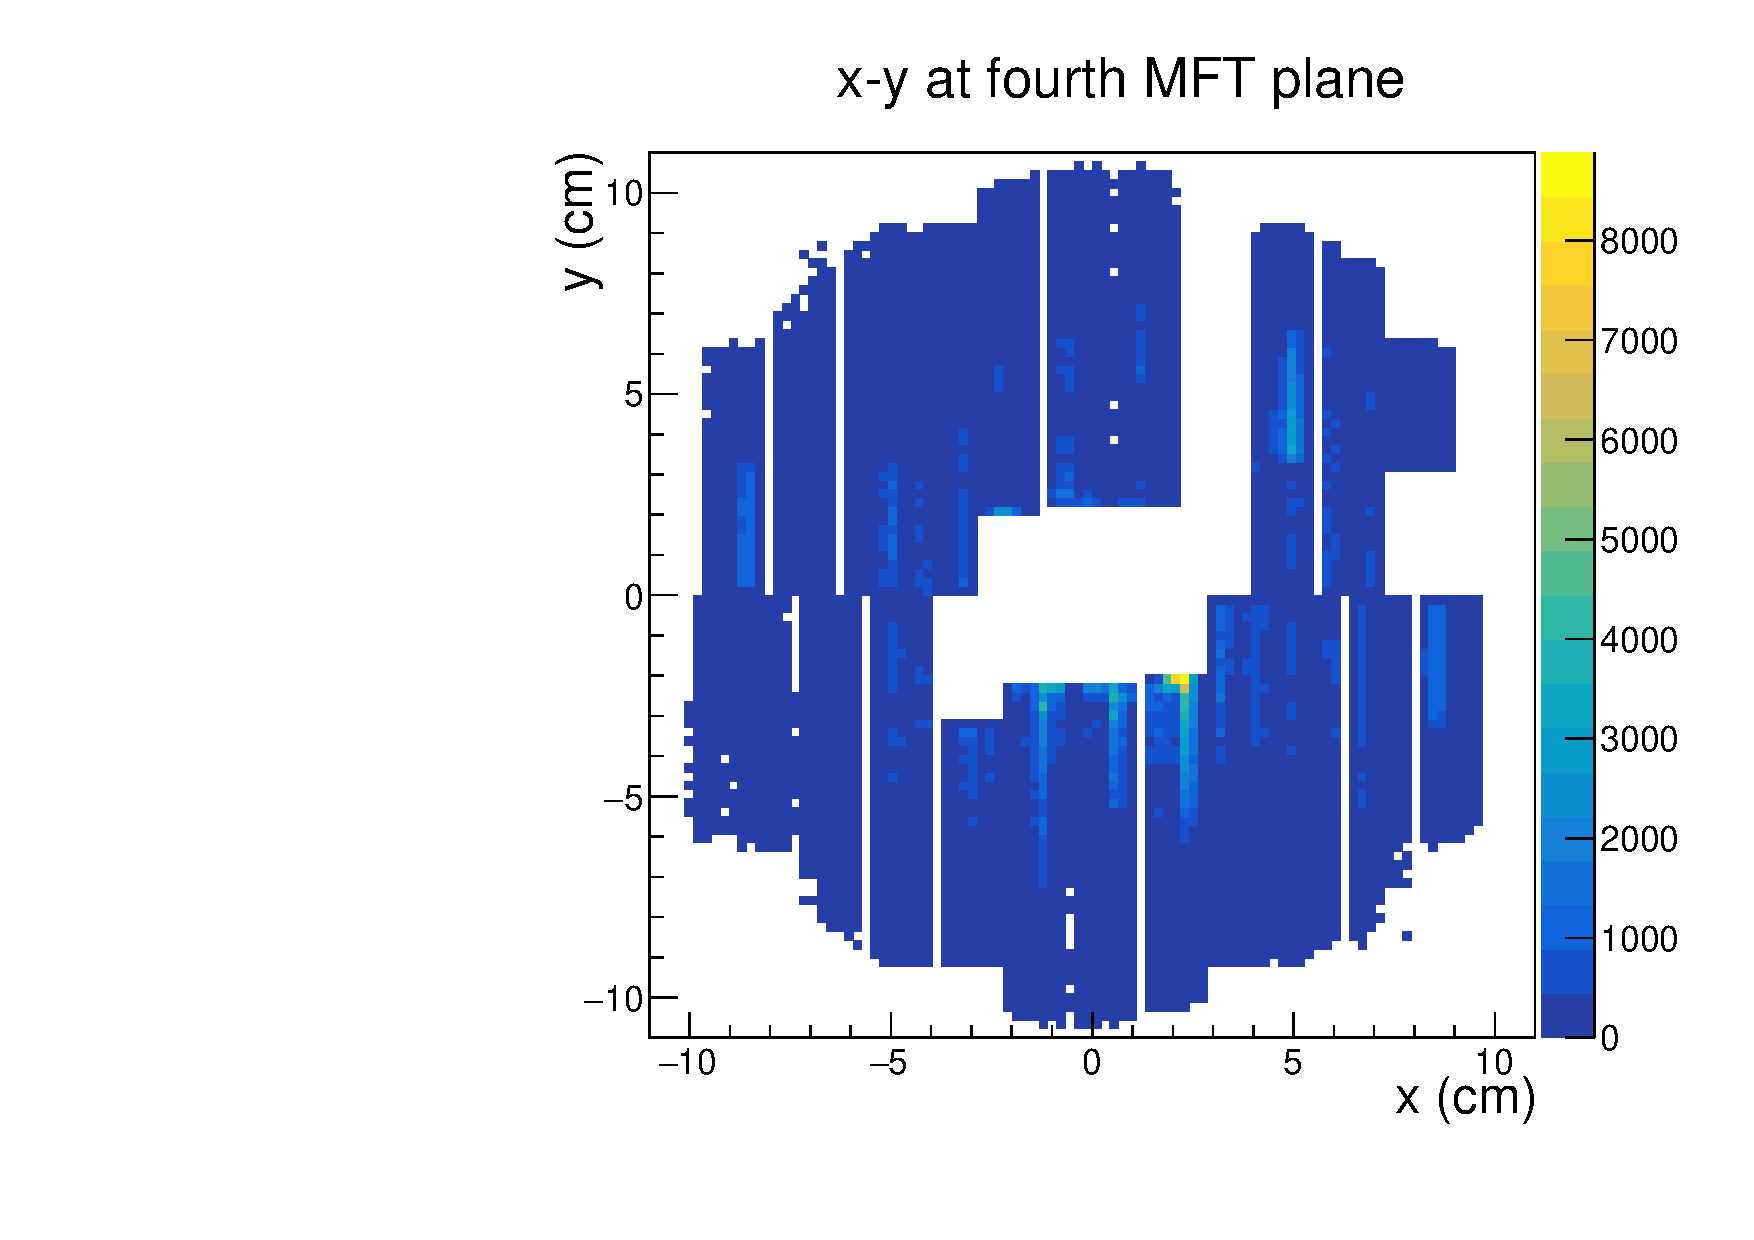
\includegraphics[width=\linewidth]{Plots/pass3_MFT/x_y_4_pass3.pdf}
        \caption{}
        \label{}
    \end{subfigure}
\caption{}
\label{fig:MFT_x_y_pass3}
\end{figure}

\subsection{Comparing pass3 to pass4}

\begin{figure}[h]%
    \centering
    \begin{subfigure}[t]{.49\linewidth}
        \centering
        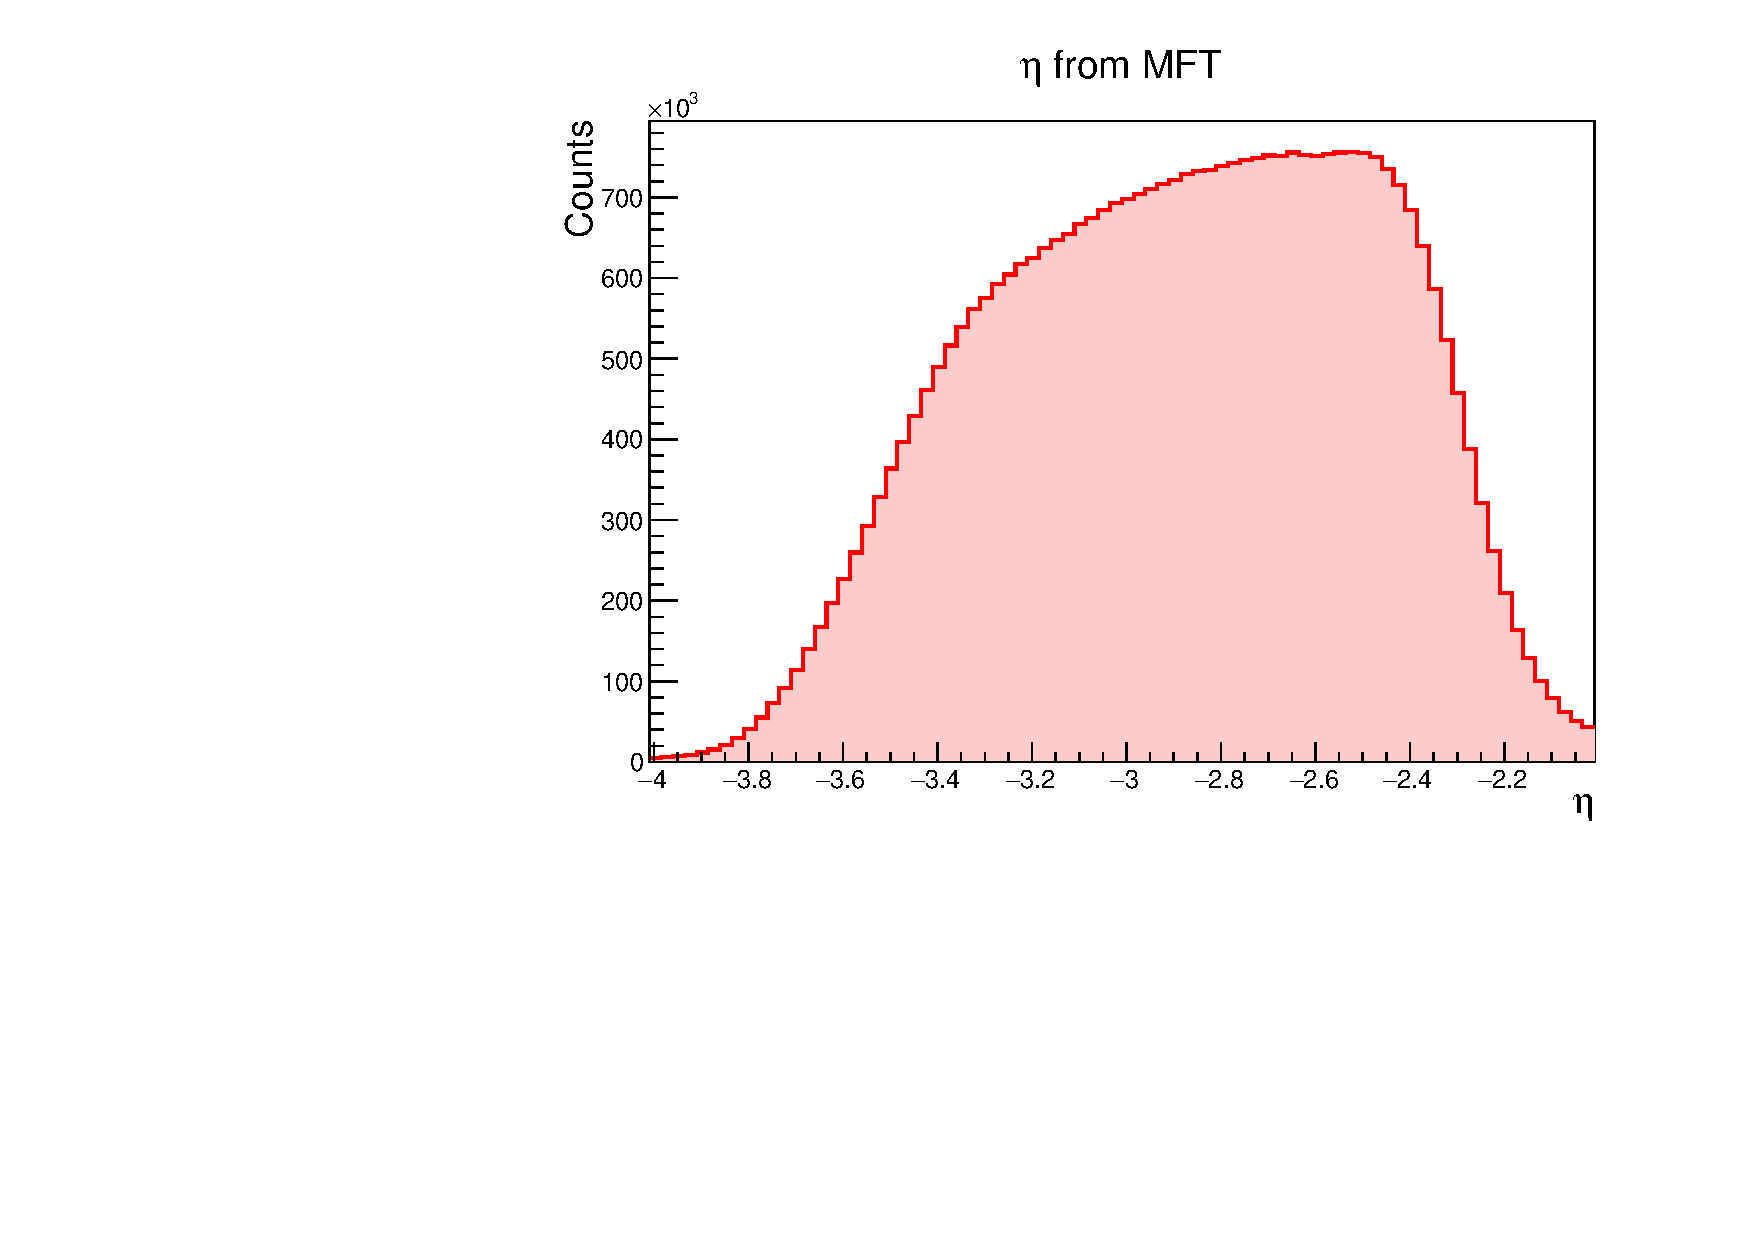
\includegraphics[width=\linewidth]{Plots/pass4_MFT/MFTeta_pass4.pdf}
        \caption{}
        \label{}
    \end{subfigure}
    \hfill
    \begin{subfigure}[t]{.49\linewidth}
        \centering
        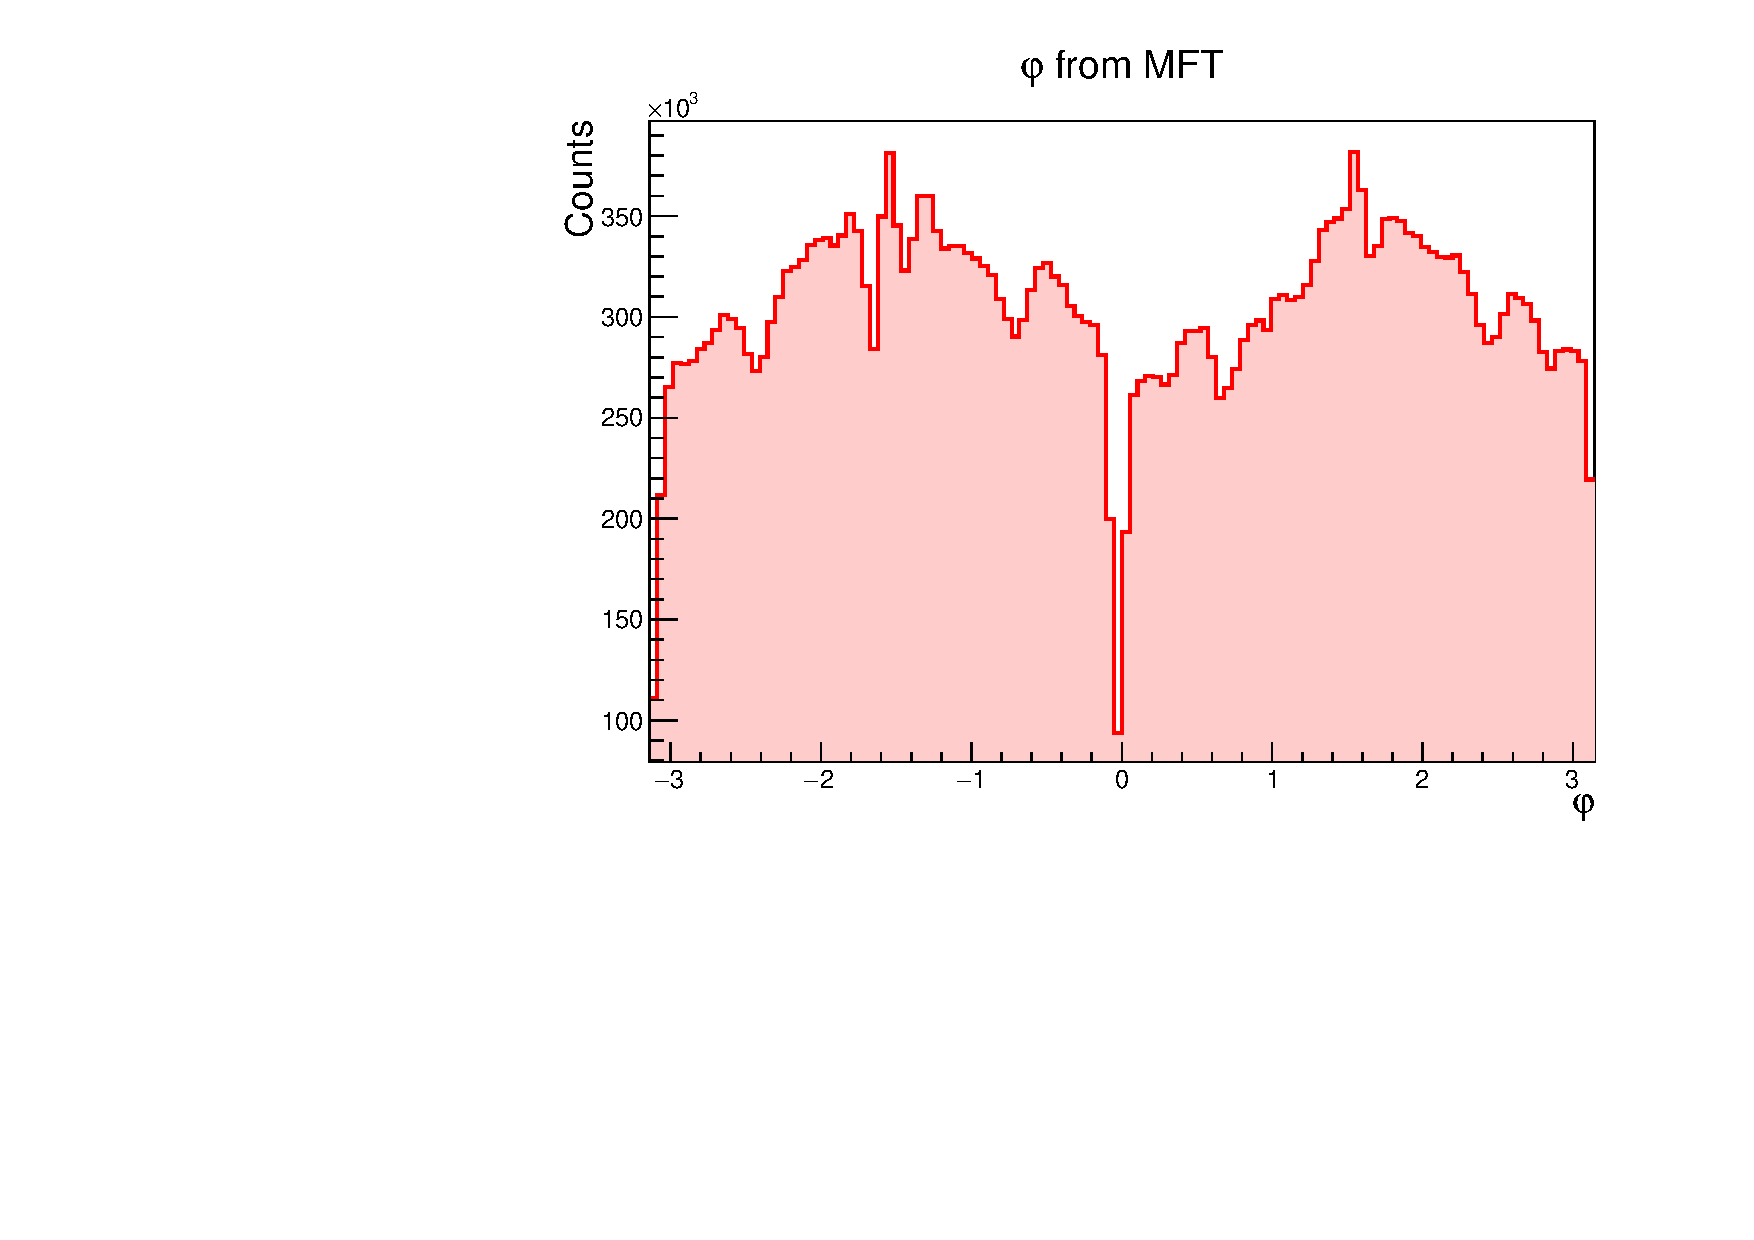
\includegraphics[width=\linewidth]{Plots/pass4_MFT/phi_pass4.pdf}
        \caption{}
        \label{}
    \end{subfigure}
    \begin{subfigure}[t]{.49\linewidth}
        \centering
        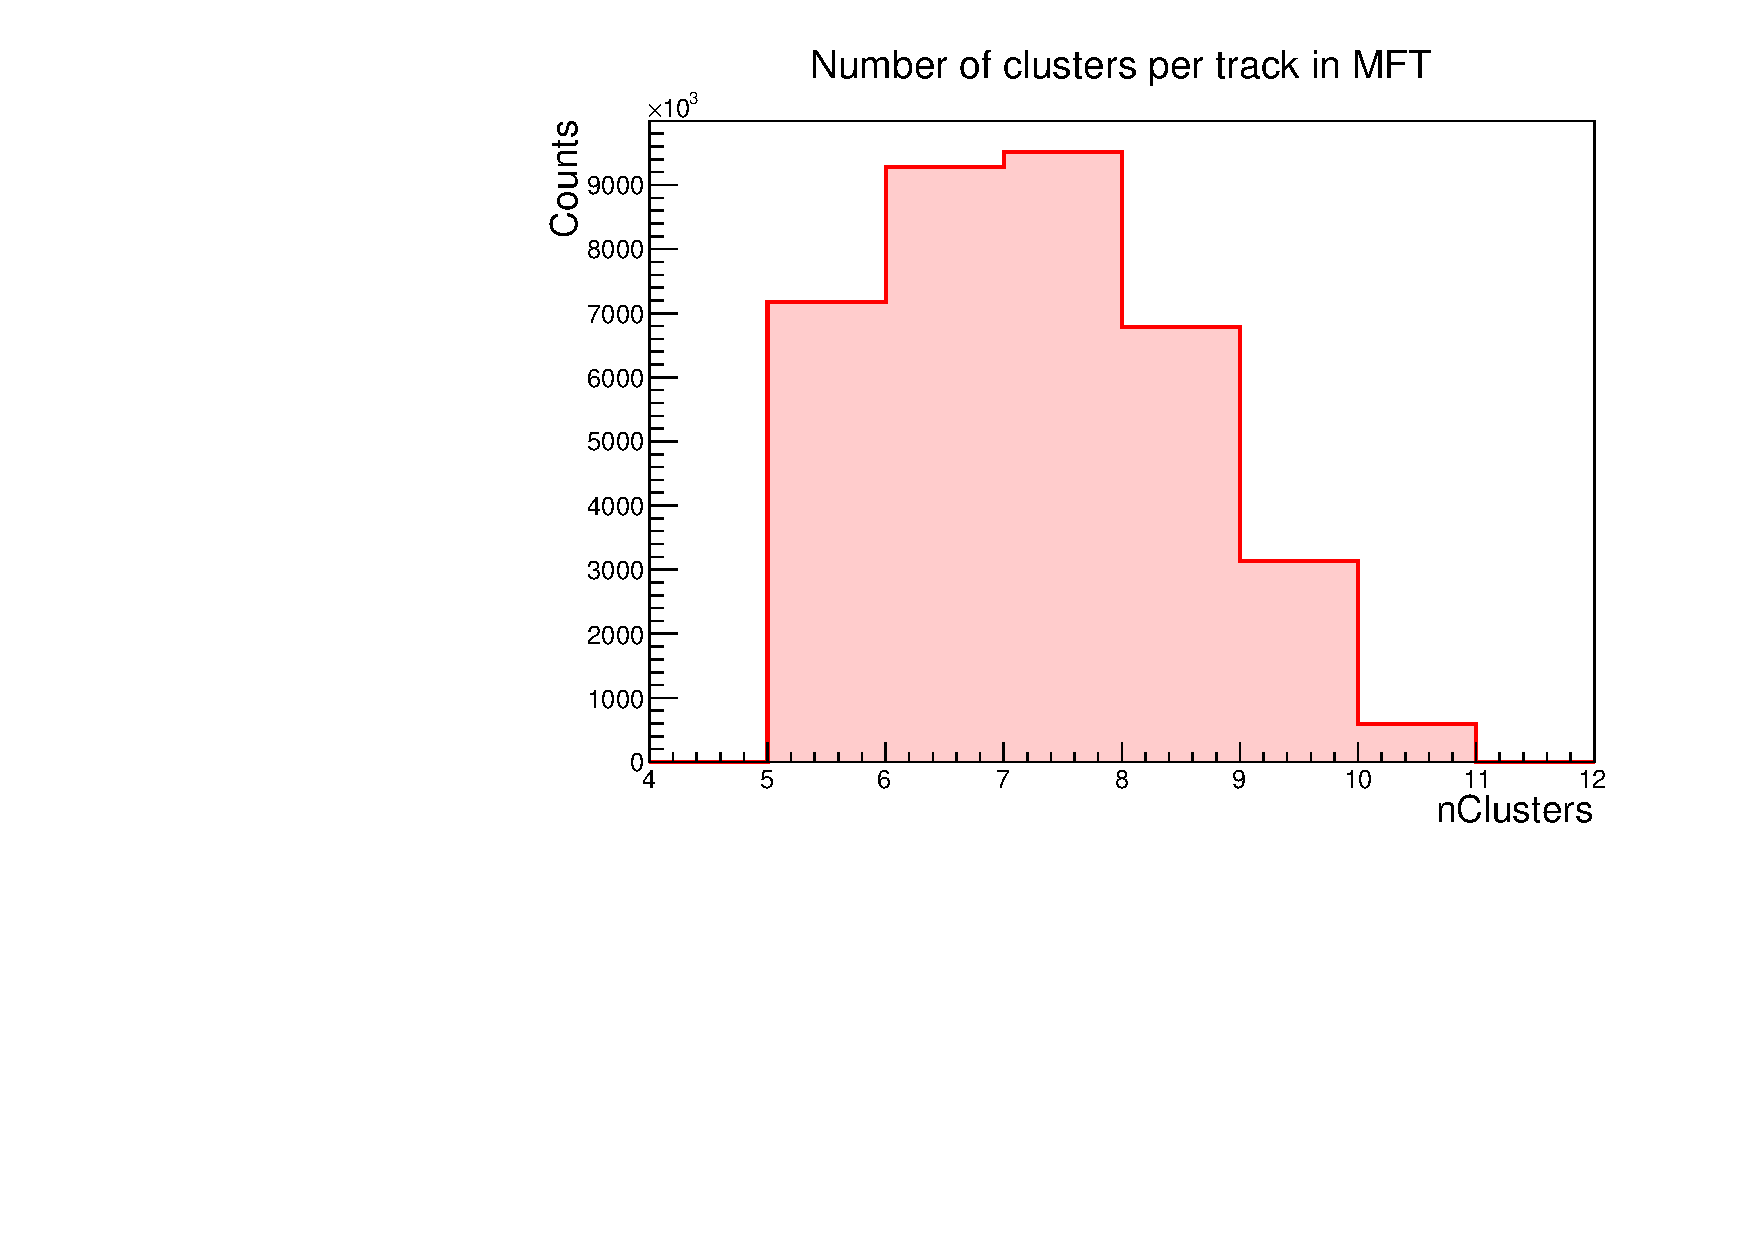
\includegraphics[width=\linewidth]{Plots/pass4_MFT/nClusters_pass4.pdf}
        \caption{}
        \label{}
    \end{subfigure}
    \hfill
    \begin{subfigure}[t]{.49\linewidth}
        \centering
        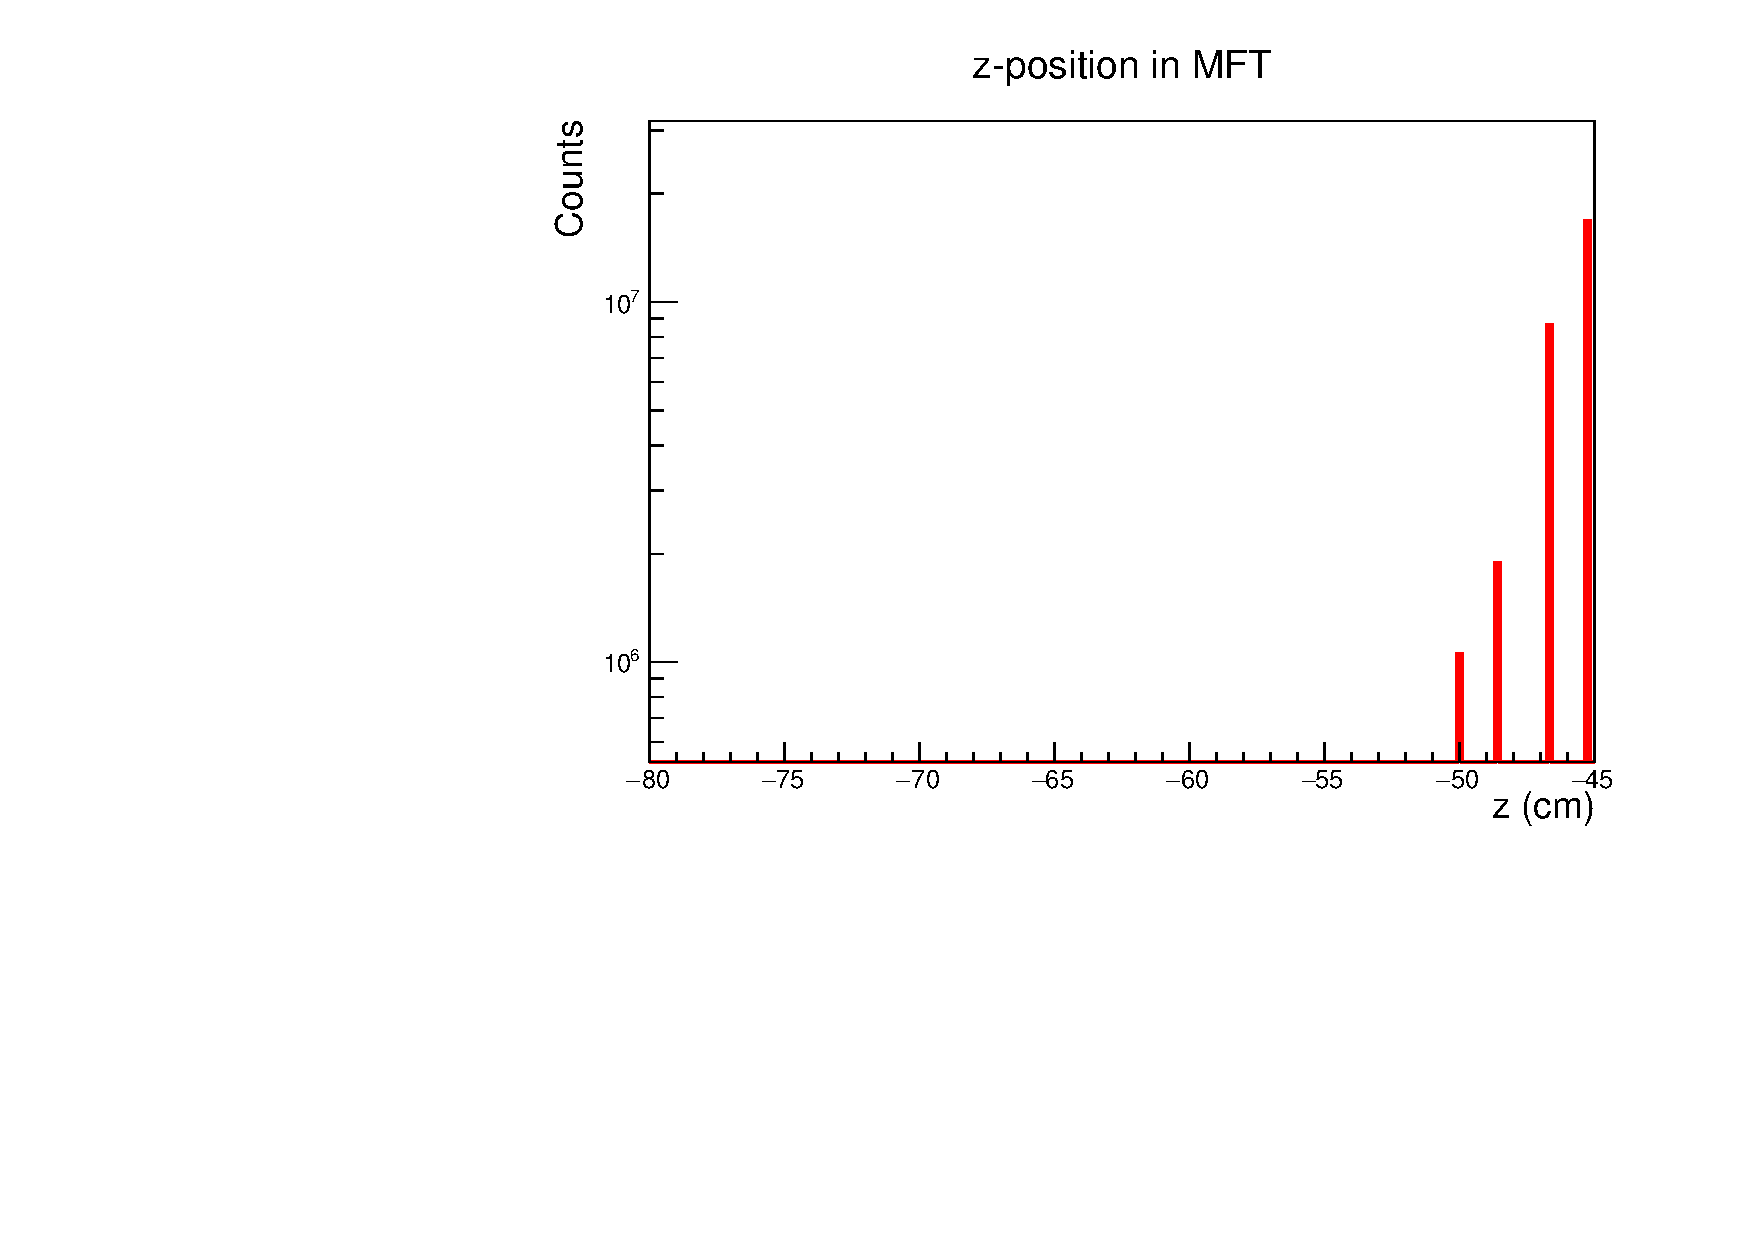
\includegraphics[width=\linewidth]{Plots/pass4_MFT/Z_MFT_pass4.pdf}
        \caption{}
        \label{}
    \end{subfigure}
\caption{}
\label{fig:MFT_1D_pass4}
\end{figure}

\begin{figure}[h]
    \begin{center}
        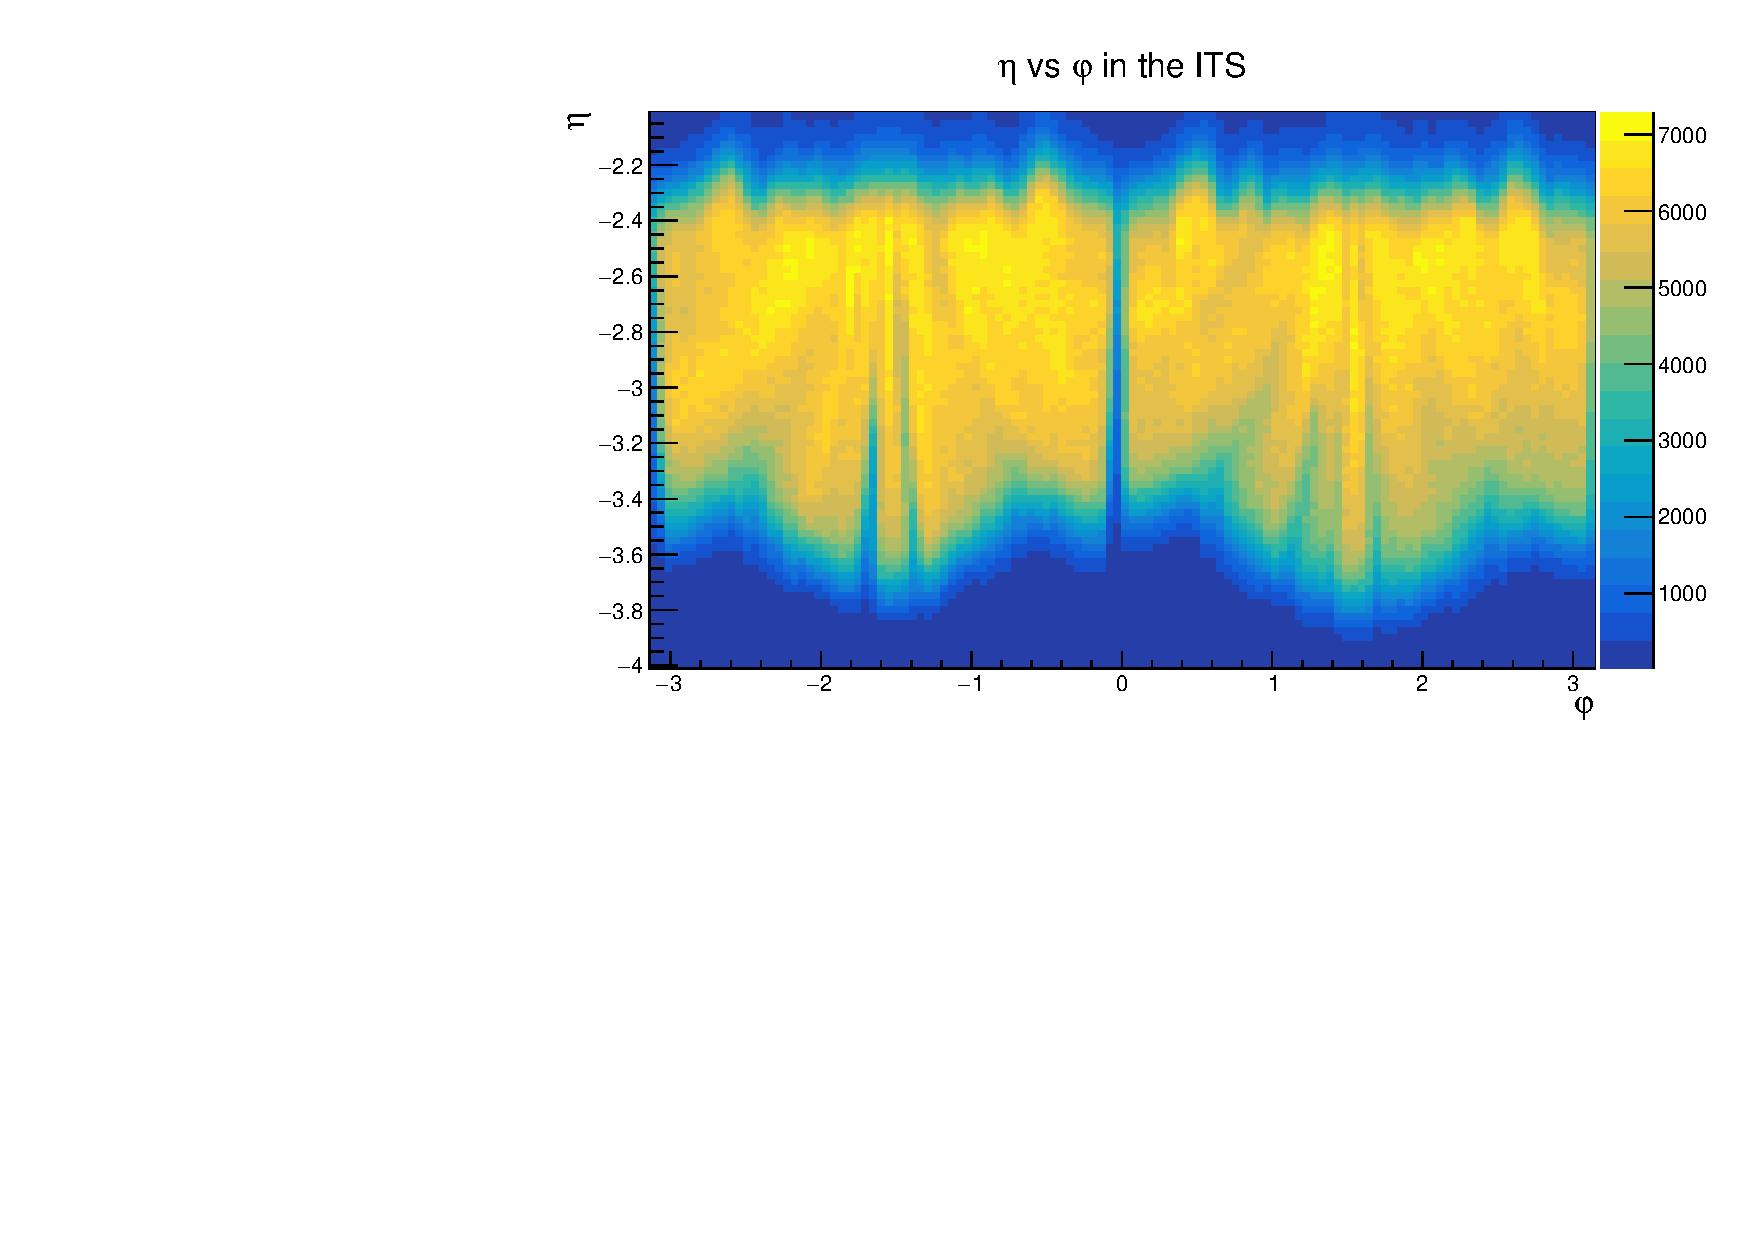
\includegraphics[width=.8\textwidth]{Plots/pass4_MFT/eta_phi_pass4.pdf}
        \caption{caption}
        \label{fig:eta_phi_pass4}
    \end{center}
\end{figure}


\begin{figure}[h]
    \begin{center}
        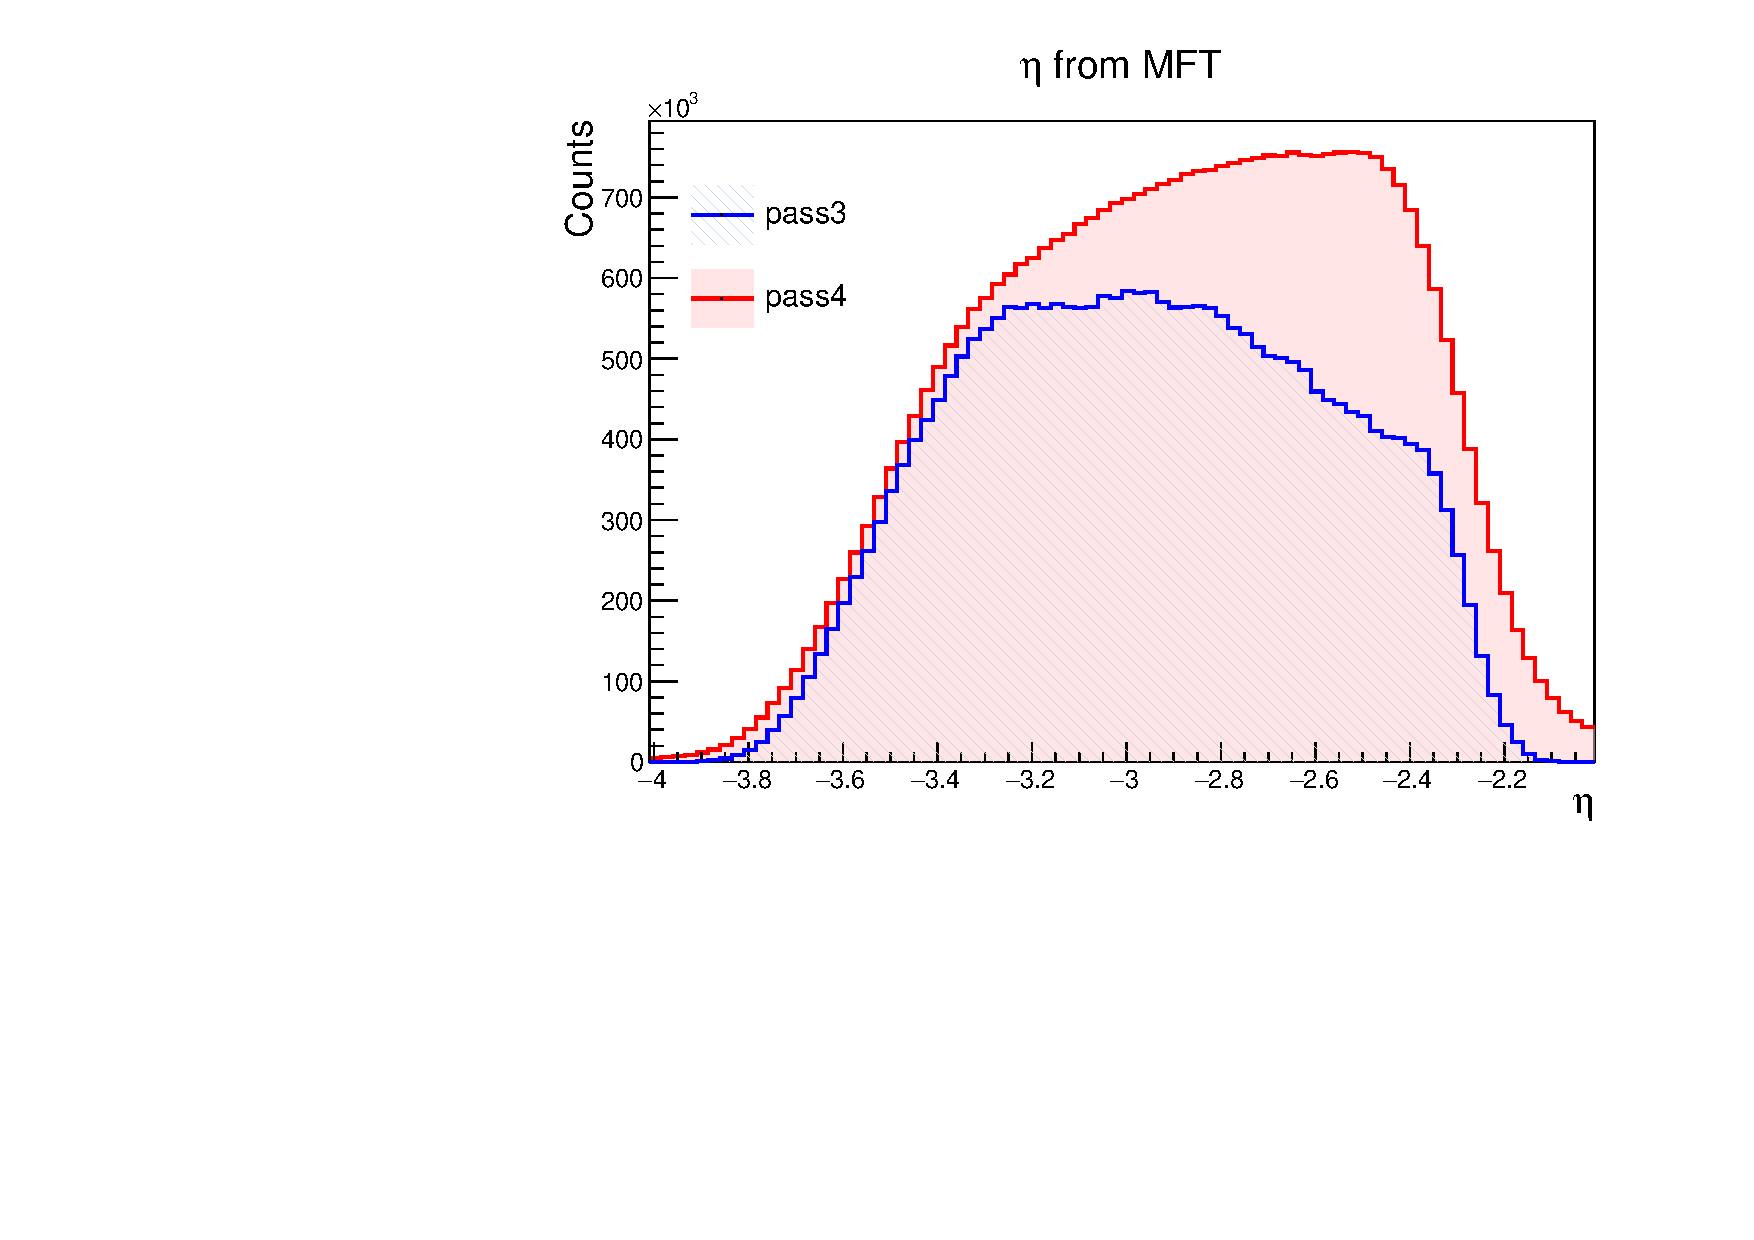
\includegraphics[width=.8\textwidth]{Plots/pass3_pass4.pdf}
        \caption{caption}
        \label{fig:pass3_pass4_eta}
    \end{center}
\end{figure}


\subsection{Initial ITS Analysis}


\subsection{Using pass4 for hasITS}